\documentclass[12pt,a4paper]{article}
\usepackage[T1]{fontenc}
\usepackage[utf8]{inputenc}
\usepackage{graphicx}
\graphicspath{{./}{Observer/reports/}{reports/}}
\usepackage{listings}
\usepackage{xcolor}
\usepackage{hyperref}
\usepackage{xurl}   % allow long URLs to break across lines
\usepackage{geometry}
\usepackage{amsmath}
\usepackage{float}

\geometry{margin=1in}
\setlength{\emergencystretch}{3em}  % avoid overfull lines from long \texttt identifiers

\definecolor{codegreen}{rgb}{0,0.6,0}
\definecolor{codegray}{rgb}{0.5,0.5,0.5}
\definecolor{codepurple}{rgb}{0.58,0,0.82}
\definecolor{backcolour}{rgb}{0.95,0.95,0.92}

\lstdefinestyle{mystyle}{
    backgroundcolor=\color{backcolour},   
    commentstyle=\color{codegreen},
    keywordstyle=\color{magenta},
    numberstyle=\tiny\color{codegray},
    stringstyle=\color{codepurple},
    basicstyle=\ttfamily\footnotesize,
    breakatwhitespace=false,         
    breaklines=true,                 
    captionpos=b,                    
    keepspaces=true,                 
    numbers=left,                    
    numbersep=5pt,                  
    showspaces=false,                
    showstringspaces=false,
    showtabs=false,                  
    tabsize=2,
    language=C++
}

\lstset{style={mystyle}}

\title{Design Pattern Report: Observer Pattern}
\author{Group 52 \\ Nguy\~{\^e}n \DJ\`inh Minh Huy (Student ID: 25125083)}
\date{\today}

\begin{document}

\maketitle
\tableofcontents
\newpage

\section{Real-world Problem}
Consider a modern financial core banking system where transactions are performed on a \texttt{BankAccount}. When a deposit occurs, several peripheral systems need to be notified of the event immediately to execute their processes:
\begin{itemize}
    \item \texttt{UI}: Updates the account balance display on the user's screen.
    \item \texttt{Email System}: Sends a transaction alert email to the customer.
    \item \texttt{Logger}: Writes transaction details to the security audit trail.
    \item \texttt{Fraud AI}: Scans transaction metadata to detect suspicious patterns.
    \item \texttt{Mobile App}: Delivers a push notification to the client's phone.
    \item \texttt{Analytics}: Records transaction metrics for business intelligence.
\end{itemize}

A customer or administrator must be able to register, enable, or disable these notification channels dynamically. The core challenge is establishing a system where a bank account can broadcast transaction updates to an arbitrary and dynamic set of observer systems without knowing their concrete classes or internal notification mechanisms.

\section{Naive Solution (Without Design Pattern)}
In a naive implementation, the \texttt{BankAccount} class holds references to concrete notification system objects directly. Below is the C++ representation of this approach:

\begin{figure}[H]
    \centering
    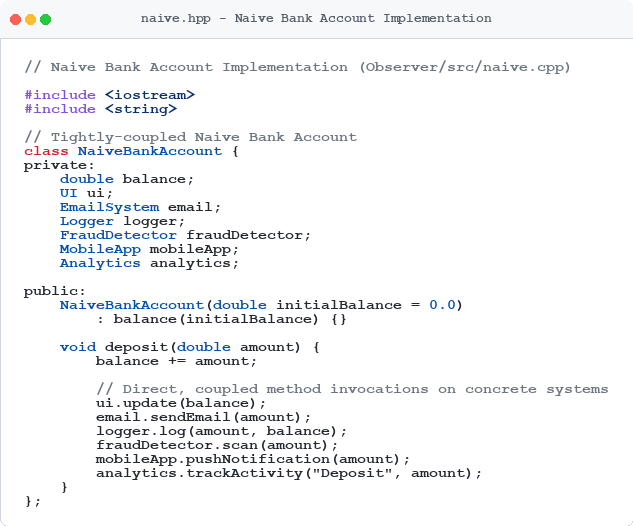
\includegraphics[width=0.9\textwidth]{naive_code_header.png}
    \caption{Naive Bank Account Header \& Implementation (\texttt{NaiveBankAccount})}
    \label{fig:naive_code_header}
\end{figure}

\begin{lstlisting}[caption=Naive Implementation of Bank Account Notifications]
// Refer to Observer/src/naive.cpp for full implementation details
class NaiveBankAccount {
private:
    double balance;
    UI ui;
    EmailSystem email;
    Logger logger;
    FraudDetector fraudDetector;
    MobileApp mobileApp;
    Analytics analytics;

public:
    NaiveBankAccount(double initialBalance) : balance(initialBalance) {}

    void deposit(double amount) {
        balance += amount;
        
        // Direct, coupled method invocations on concrete systems
        ui.update(balance);
        email.sendEmail(amount);
        logger.log(amount, balance);
        fraudDetector.scan(amount);
        mobileApp.pushNotification(amount);
        analytics.trackActivity("Deposit", amount);
    }
};
\end{lstlisting}

\begin{figure}[H]
    \centering
    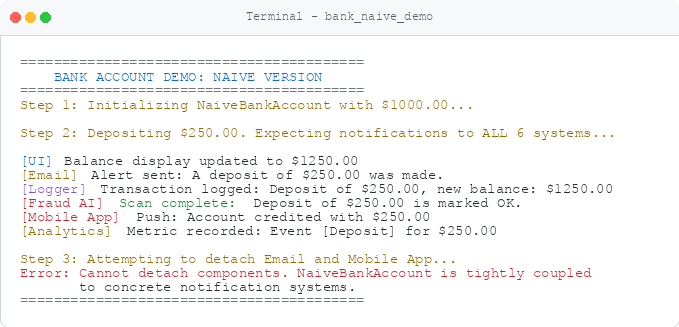
\includegraphics[width=0.8\textwidth]{naive_console_output.png}
    \caption{Console Output of the Naive Bank Account Demo (No Observer Pattern)}
    \label{fig:naive_console_output}
\end{figure}

\section{Problems with the Naive Solution}
The naive approach exhibits several major architectural flaws:
\begin{enumerate}
    \item \textbf{Tight Coupling:} The \texttt{NaiveBankAccount} is tightly coupled to concrete classes like \texttt{UI}, \texttt{EmailSystem}, \texttt{Logger}, \texttt{FraudDetector}, \texttt{MobileApp}, and \texttt{Analytics}. It must know their names, structures, and exactly which update method to call on each.
    \item \textbf{Violation of the Open-Closed Principle (OCP):} If we want to introduce a new system (such as a compliance reporting system or a credit score monitoring engine), we must modify the core \texttt{NaiveBankAccount} class. This requires adding a new member field and updating the notification logic inside the \texttt{deposit} method.
    \item \textbf{Violation of the Single Responsibility Principle (SRP):} The \texttt{BankAccount} class should focus solely on financial ledger operations (managing the balance and transactions). However, it is also burdened with orchestrating emails, logs, mobile push notifications, and security analysis.
\end{enumerate}

\section{Introduction to the Observer Pattern}
The \textbf{Observer Pattern} is a behavioral design pattern that defines a one-to-many dependency between objects. When one object (the \textbf{Subject} or \textbf{Publisher}) changes state, all its dependents (the \textbf{Observers} or \textbf{Subscribers}) are notified and updated automatically.

Key concepts:
\begin{itemize}
    \item \textbf{Subject:} Knows its observers and provides an interface to attach or detach them.
    \item \textbf{Observer:} Defines an updating interface for objects that should be notified.
    \item \textbf{ConcreteSubject:} Stores state of interest to ConcreteObservers and sends notifications.
    \item \textbf{ConcreteObserver:} Implements the Observer updating interface to keep its state consistent with the subject.
\end{itemize}

\section{General Class Diagram}
In the general Observer pattern structure:
\begin{itemize}
    \item A \texttt{Subject} maintains a list of references to \texttt{Observer} objects.
    \item The \texttt{Subject} exposes interfaces: \texttt{attach(Observer)}, \texttt{detach(Observer)}, and \texttt{notify()}.
    \item \texttt{Observer} exposes the \texttt{update()} method interface.
\end{itemize}

\begin{figure}[H]
    \centering
    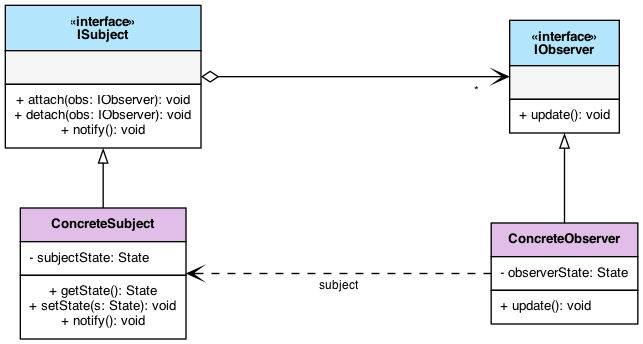
\includegraphics[width=0.85\textwidth]{general_observer_uml.png}
    \caption{General Observer Design Pattern UML Diagram}
    \label{fig:general_uml}
\end{figure}

\section{Class Diagram for the Bank Account Problem}
Applying the pattern to our problem:
\begin{itemize}
    \item \texttt{BankAccount} acts as the ConcreteSubject (or subject coordinator).
    \item \texttt{AccountObserver} acts as the Observer interface.
    \item The ConcreteObservers each implement \texttt{onTransaction()} and react on their own terms:
    \begin{itemize}
        \item \texttt{UIObserver} -- refreshes the on-screen balance.
        \item \texttt{EmailObserver} -- sends the transaction alert email.
        \item \texttt{LoggerObserver} -- writes the security audit trail.
        \item \texttt{FraudAIObserver} -- warns on suspicious amounts.
        \item \texttt{MobileAppObserver} -- delivers the push notification.
        \item \texttt{AnalyticsObserver} -- records the business metric.
    \end{itemize}
\end{itemize}

\begin{figure}[H]
    \centering
    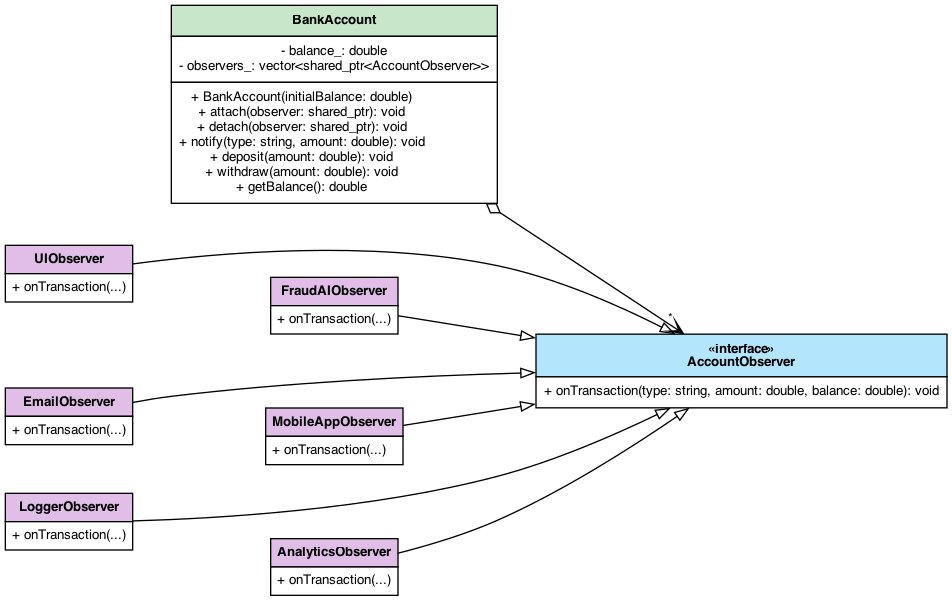
\includegraphics[width=0.95\textwidth]{bank_observer_uml.png}
    \caption{UML Class Diagram for Bank Account Notification System}
    \label{fig:bank_uml}
\end{figure}

\section{Implementation of the Observer Pattern}
By decoupling the classes through abstract interfaces, our refactored implementation allows adding or removing subscriber systems at runtime without modifying the core subject.

\begin{figure}[H]
    \centering
    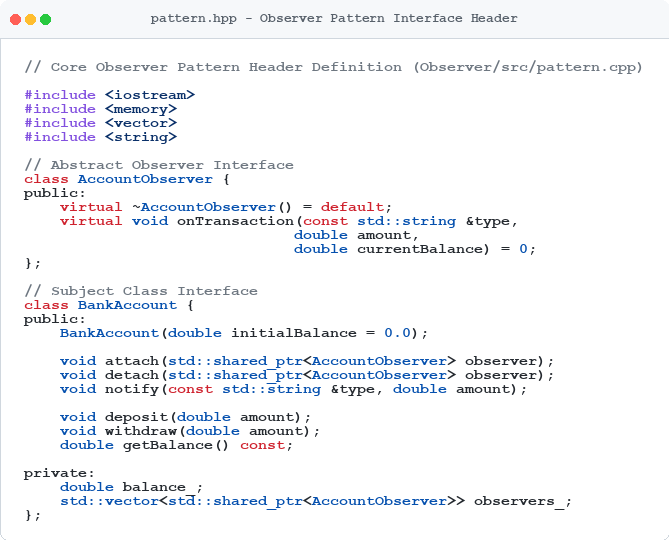
\includegraphics[width=0.9\textwidth]{pattern_code_header.png}
    \caption{Core Header Definition of the Observer Pattern Interface (\texttt{AccountObserver} and \texttt{BankAccount})}
    \label{fig:pattern_code_header}
\end{figure}

\begin{figure}[H]
    \centering
    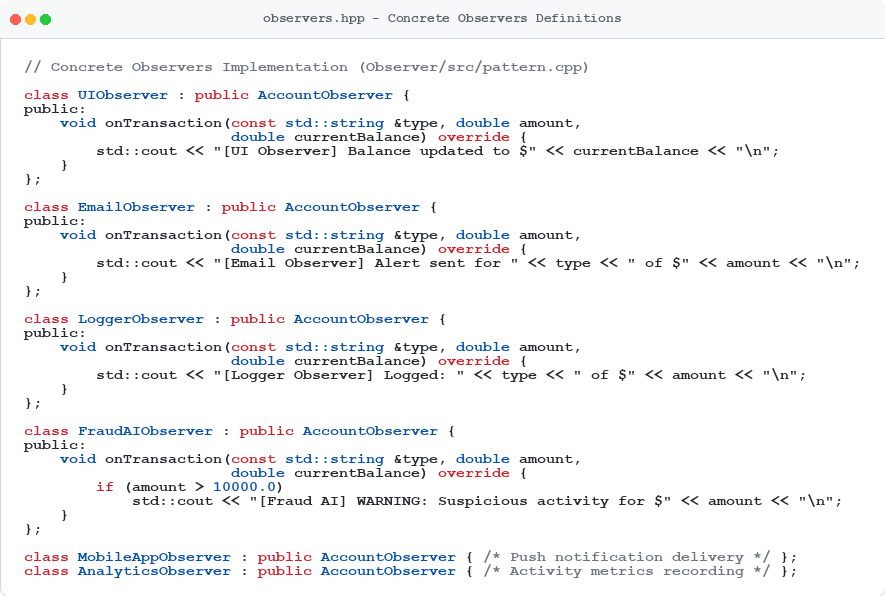
\includegraphics[width=0.9\textwidth]{concrete_observers_header.png}
    \caption{Implementation Header of Concrete Observer Subscribers}
    \label{fig:concrete_observers_header}
\end{figure}

\begin{lstlisting}[caption=Refactored Observer Implementation]
// Refer to Observer/src/pattern.cpp for full implementation details
class AccountObserver {
public:
    virtual ~AccountObserver() = default;
    virtual void onTransaction(const std::string &type, double amount,
                               double currentBalance) = 0;
};

class BankAccount {
public:
    BankAccount(double initialBalance = 0.0) : balance_(initialBalance) {}

    void attach(std::shared_ptr<AccountObserver> observer) {
        observers_.push_back(observer);
    }
    void detach(std::shared_ptr<AccountObserver> observer) {
        observers_.erase(
            std::remove(observers_.begin(), observers_.end(), observer),
            observers_.end());
    }
    void notify(const std::string &type, double amount) {
        for (auto observer : observers_) {
            observer->onTransaction(type, amount, balance_);
        }
    }

    void deposit(double amount) {
        balance_ += amount;
        notify("Deposit", amount);
    }
    void withdraw(double amount) {
        if (amount > balance_) {
            notify("FailedWithdrawal", amount);   // rejected: insufficient funds
        } else {
            balance_ -= amount;
            notify("Withdrawal", amount);
        }
    }

    double getBalance() const { return balance_; }

private:
    double balance_;
    std::vector<std::shared_ptr<AccountObserver>> observers_;
};
\end{lstlisting}

\begin{figure}[H]
    \centering
    \begin{minipage}[t]{0.49\textwidth}
        \centering
        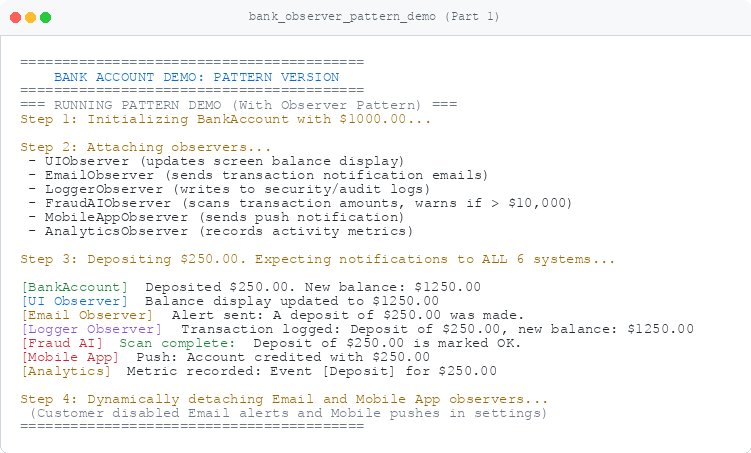
\includegraphics[width=\textwidth]{pattern_console_output_1.png}
        \caption{Refactored Demo Output -- Part 1}
        \label{fig:pattern_console_1}
    \end{minipage}
    \hfill
    \begin{minipage}[t]{0.49\textwidth}
        \centering
        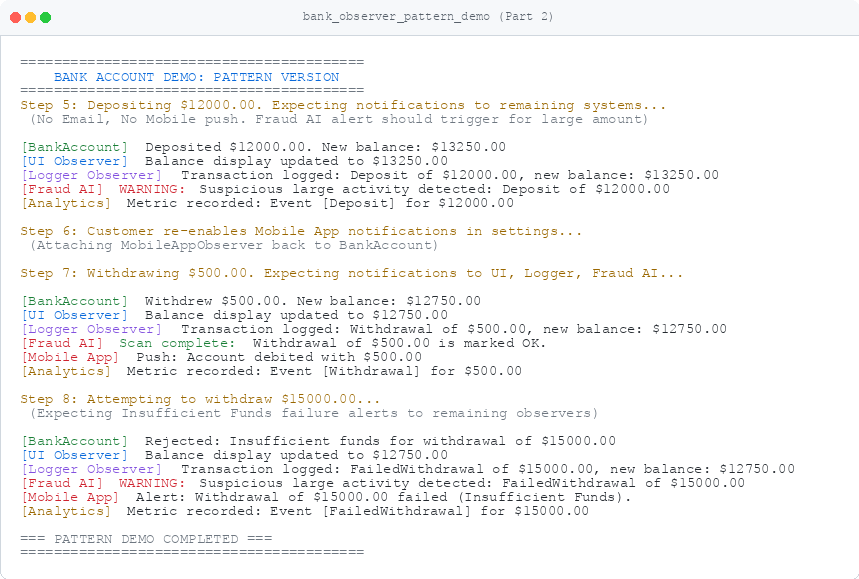
\includegraphics[width=\textwidth]{pattern_console_output_2.png}
        \caption{Refactored Demo Output -- Part 2}
        \label{fig:pattern_console_2}
    \end{minipage}
\end{figure}

\begin{figure}[H]
    \centering
    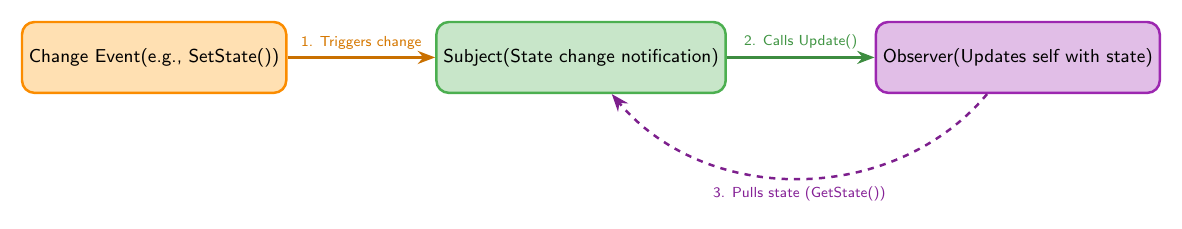
\includegraphics[width=0.7\textwidth]{observer_flowchart_1.png}
    \caption{Sequential Process Flowchart of a Single Observer Notification}
    \label{fig:observer_flowchart_1}
\end{figure}

\begin{figure}[H]
    \centering
    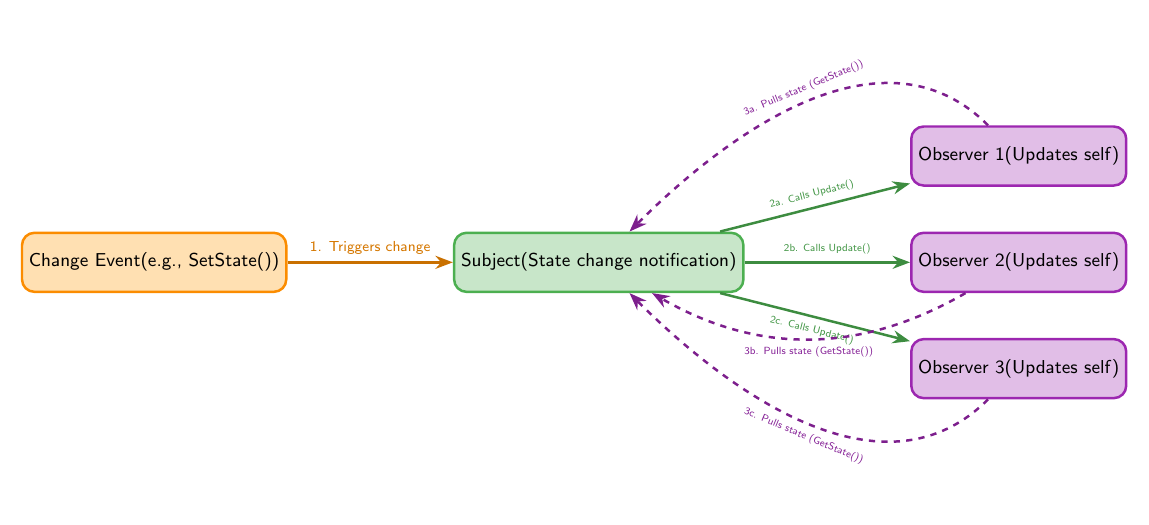
\includegraphics[width=0.85\textwidth]{observer_flowchart_many.png}
    \caption{Sequential Process Flowchart with Multiple Observers (Pull Model)}
    \label{fig:observer_flowchart_many}
\end{figure}

\begin{figure}[H]
    \centering
    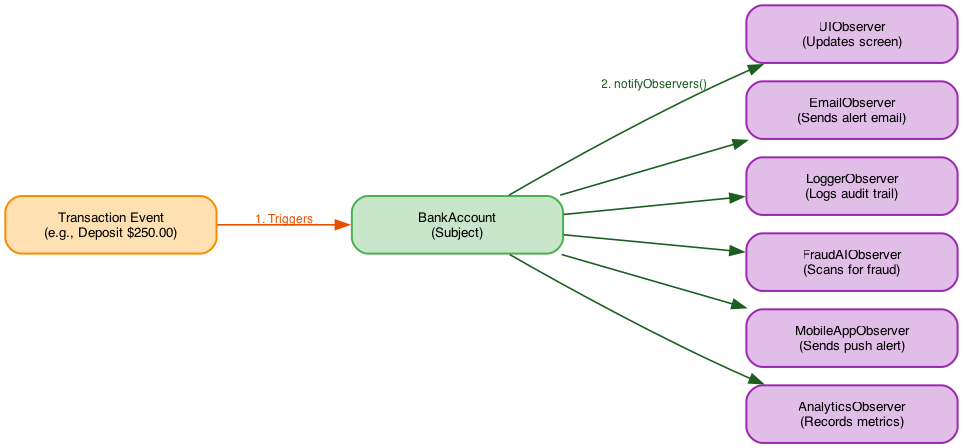
\includegraphics[width=0.95\textwidth]{observer_flowchart_bank.png}
    \caption{Process Flowchart for Bank Account Notification System (Push Model)}
    \label{fig:observer_flowchart_bank}
\end{figure}

\section{Pros and Cons}
\subsection{Pros}
\begin{itemize}
    \item \textbf{Loose Coupling:} The Subject and Observers are loosely coupled. The Subject only knows that the observer implements a specific interface.
    \item \textbf{Support for Broadcast Communication:} Unlike direct calls, notifications are broadcast automatically to all registered subscribers.
    \item \textbf{Open-Closed Principle:} We can introduce new concrete observer classes without changing the subject's code.
\end{itemize}

\subsection{Cons}
\begin{itemize}
    \item \textbf{Lapsed Listener Problem:} Observers must be carefully deregistered when destroyed, or they remain in memory and get called, causing undefined behavior or leaks.
    \item \textbf{Unintended Update Chains:} If observers trigger updates on subjects, it can lead to complex and hard-to-debug cascading updates or infinite loops.
    \item \textbf{Ordering Concerns:} There is no guarantee in which order the observers will be notified.
\end{itemize}

\section{Other Real-world Applications}
\subsection{Web Development}
\begin{itemize}
    \item \textbf{Event Handling in JavaScript:} The DOM's \texttt{addEventListener} uses the Observer pattern to attach event handlers to HTML elements.
    \item \textbf{State Management (Redux/Vuex):} Views subscribe to changes in a global store and re-render automatically when state mutations occur.
\end{itemize}
\subsection{Mobile Development}
\begin{itemize}
    \item \textbf{RxSwift / RxJava / RxKotlin:} Reactive streams rely heavily on observing data sequences and binding them directly to UI components.
    \item \textbf{SwiftUI/Android Jetpack Compose:} Declarative UI frameworks use property wrappers like \texttt{@Published} and state flows to push model updates directly to the view.
\end{itemize}

\section{Observer and Mediator Fusion}
In complex system architectures, the \textit{Observer} and \textit{Mediator} patterns are frequently fused together to handle coordination and communication between multiple components. 

In a standard Mediator implementation, colleagues must explicitly call the mediator, and the mediator directly invokes actions on other colleagues. By fusing the two patterns:
\begin{itemize}
    \item \textbf{Colleagues act as Subjects:} They maintain state and notify registered observers when changes occur, remaining completely unaware of who is listening.
    \item \textbf{The Mediator acts as an Observer:} It subscribes to the event streams of the Colleagues. When it receives an \texttt{update()} notification, it coordinates and executes the required reaction across other Colleagues.
\end{itemize}
This fusion achieves dynamic event-driven routing while preserving loose coupling between Colleagues.

\begin{figure}[H]
    \centering
    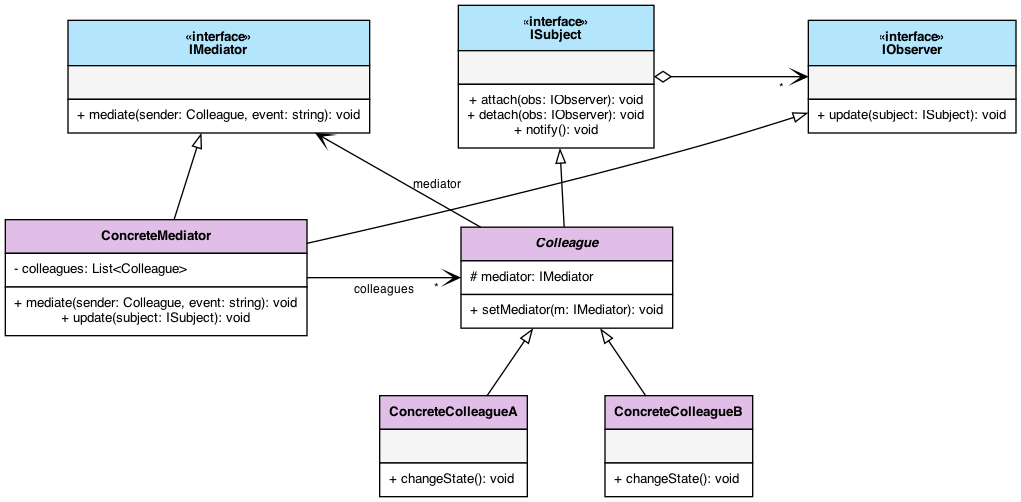
\includegraphics[width=0.9\textwidth]{observer_mediator_uml.png}
    \caption{UML Class Diagram of the Observer-Mediator Fusion}
    \label{fig:observer_mediator_uml}
\end{figure}

\begin{figure}[H]
    \centering
    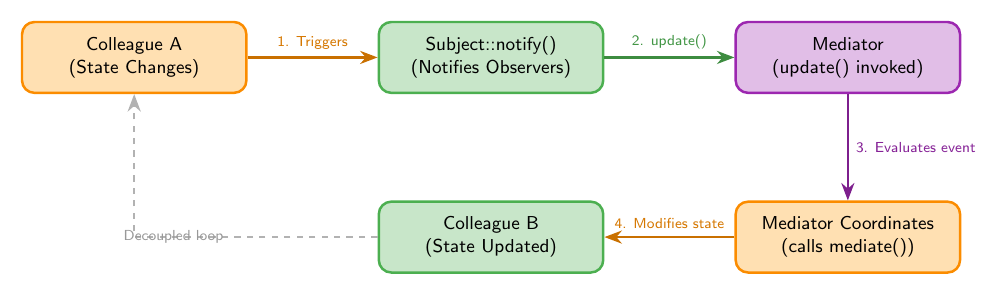
\includegraphics[width=0.85\textwidth]{observer_mediator_flowchart.png}
    \caption{Process Flowchart of Event-Driven Mediation Flow}
    \label{fig:observer_mediator_flowchart}
\end{figure}

\subsection{Case Study: Super Mario Game EventBus}
In game development, handling interactions between numerous entities and systems (e.g., updating UI when a player dies, unlocking achievements when a coin is collected, playing sounds when blocks break) can easily lead to spaghetti code and tight coupling. To solve this, a decentralized event-routing system known as an \textbf{EventBus} is used.

The \texttt{EventBus} acts as a central singleton \textit{Mediator}. Colleagues (such as the \texttt{Player} or \texttt{POWBlock}) publish events to the \texttt{EventBus} without knowing who reacts to them. Other systems (such as the \texttt{StatisticsTracker} or \texttt{AchievementManager}) register as \textit{Observers} to specific event types.

\begin{figure}[H]
    \centering
    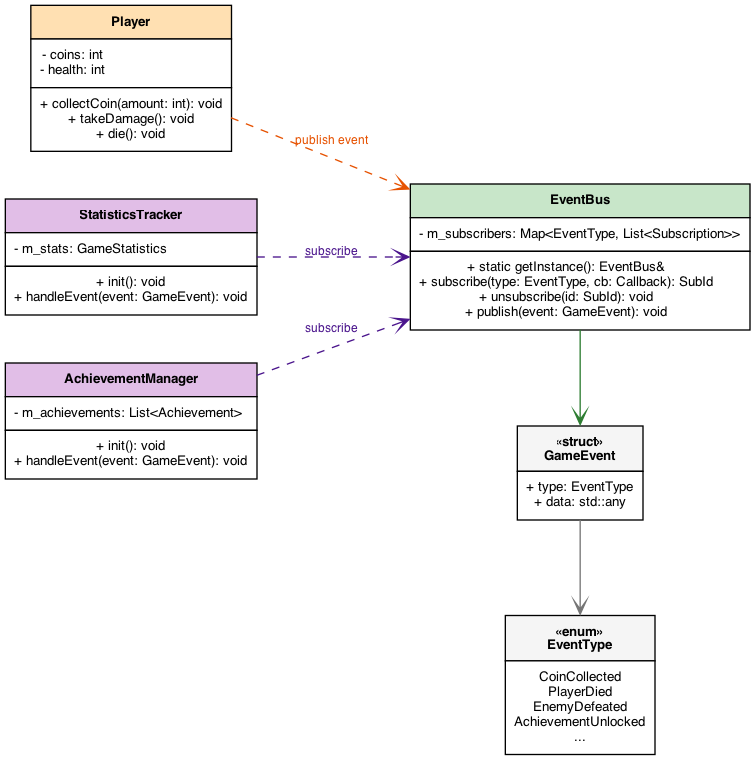
\includegraphics[width=0.9\textwidth]{mario_eventbus_uml.png}
    \caption{UML Class Diagram for Super Mario Game EventBus System}
    \label{fig:mario_eventbus_uml}
\end{figure}

The C++ interface for the game's EventBus is implemented as follows:
\begin{lstlisting}[language=C++]
// include/Core/EventBus.hpp
class EventBus {
public:
  using Callback = std::function<void(const GameEvent &)>;
  using SubscriptionId = size_t;

  // Singleton Instance access
  static EventBus &getInstance();

  // Event operations (Mediating Hub)
  SubscriptionId subscribe(EventType type, Callback callback);
  void unsubscribe(SubscriptionId id);
  void publish(const GameEvent &event);

private:
  EventBus() = default;
  
  struct Subscription {
    SubscriptionId id;
    Callback callback;
  };

  std::unordered_map<EventType, std::vector<Subscription>> m_subscribers;
  SubscriptionId m_nextId = 0;
};
\end{lstlisting}

\begin{figure}[H]
    \centering
    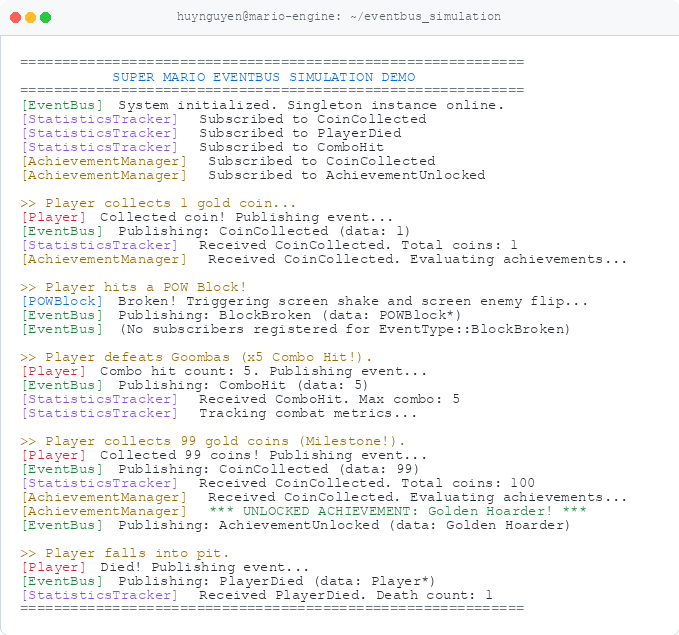
\includegraphics[width=0.95\textwidth]{mario_eventbus_demo.png}
    \caption{Console Output Simulation of EventBus Event-Driven Mediation}
    \label{fig:mario_eventbus_demo}
\end{figure}

\section{Observer and Interpreter Fusion}
The \textit{Interpreter} pattern represents a sentence of a language as a tree of expression objects, where every node knows how to solve itself and delegates to its children. This works cleanly while every leaf is a constant: the tree is built once and evaluated once.

The situation changes when a terminal expression is a \textbf{variable} that another process, service, or user can rewrite. Every result computed above that leaf immediately becomes stale, and the tree has no way of knowing. Polling the whole tree for changes is exactly the waste the Observer pattern was designed to eliminate.

By fusing the two patterns:
\begin{itemize}
    \item \textbf{The variable node acts as the Subject:} it notifies its subscribers whenever its value is rewritten.
    \item \textbf{The dependent expressions act as Observers:} on notification, only the affected branch is re-evaluated, leaving the rest of the tree untouched.
\end{itemize}

\subsection{Case Study: Spreadsheet Formula Cells}
Consider a spreadsheet in which cell \texttt{A3} holds the formula \texttt{= A1 + A2}. The Interpreter pattern parses that formula into an expression tree, while the Observer pattern keeps the result synchronised: \texttt{A3} subscribes to \texttt{A1} and \texttt{A2}, so rewriting either cell -- by another formula or by the user -- triggers an immediate re-interpretation of \texttt{A3} alone.

\begin{lstlisting}[caption=Observing a Mutable Terminal Expression]
class Expression {
public:
    virtual ~Expression() = default;
    virtual double solve() const = 0;
};

class ExpressionObserver {
public:
    virtual ~ExpressionObserver() = default;
    virtual void onValueChanged() = 0;
};

// A terminal expression that other components may rewrite: the Subject
class VariableExpression : public Expression {
public:
    explicit VariableExpression(double value) : value_(value) {}

    double solve() const override { return value_; }

    void attach(std::weak_ptr<ExpressionObserver> observer) {
        observers_.push_back(std::move(observer));
    }
    void setValue(double value) {
        value_ = value;
        notify();
    }

private:
    void notify() {
        // weak_ptr expires with the observer, avoiding the lapsed listener problem
        for (const auto &weak : observers_) {
            if (auto observer = weak.lock()) {
                observer->onValueChanged();
            }
        }
    }

    double value_;
    std::vector<std::weak_ptr<ExpressionObserver>> observers_;
};

// Cell A3: holds the parsed tree for "= A1 + A2" and observes both leaves
class FormulaCell : public ExpressionObserver {
public:
    explicit FormulaCell(std::shared_ptr<Expression> formula)
        : formula_(std::move(formula)), cached_(formula_->solve()) {}

    void onValueChanged() override { cached_ = formula_->solve(); }

    double value() const { return cached_; }

private:
    std::shared_ptr<Expression> formula_;
    double cached_;
};
\end{lstlisting}

The same fusion drives automated trading rules: the Interpreter parses a user-written condition such as \texttt{price > 100 AND volume > 500}, while the Observer pattern broadcasts market updates that trigger the rule evaluation.

\section{Quiz}
Here are some interactive questions to review the Observer pattern:

\begin{enumerate}
    \item What type of design pattern is the Observer Pattern?
    \begin{itemize}
        \item[A)] Creational
        \item[B)] Structural
        \item[C)] Behavioral
        \item[D)] Architectural
    \end{itemize}
    
    \item Which SOLID principle does the Observer pattern primarily help satisfy when adding new subscribers?
    \begin{itemize}
        \item[A)] Liskov Substitution Principle
        \item[B)] Single Responsibility Principle
        \item[C)] Interface Segregation Principle
        \item[D)] Open-Closed Principle
    \end{itemize}

    \item What is the ``Lapsed Listener'' problem in the Observer pattern?
    \begin{itemize}
        \item[A)] The subject stops listening to updates.
        \item[B)] Observers are not notified because the subject crashed.
        \item[C)] An observer is deleted without unsubscribing, causing memory leaks/crashes.
        \item[D)] Multiple subjects occupy the same listener list.
    \end{itemize}

    \item Which of the following is a key advantage of the Observer pattern?
    \begin{itemize}
        \item[A)] It ensures observers are updated sequentially.
        \item[B)] It decouples the subject from concrete observer details.
        \item[C)] It reduces memory overhead of notifications.
        \item[D)] It prevents subjects from changing their state.
    \end{itemize}

    \item In the \textit{pull} model of the Observer pattern, what does the subject send to its observers?
    \begin{itemize}
        \item[A)] All of the changed data, packaged inside the notification.
        \item[B)] Only the announcement that its state changed; each observer then fetches what it needs through getters.
        \item[C)] Nothing -- observers poll the subject on a timer instead.
        \item[D)] A notification to the first registered observer only.
    \end{itemize}

    \item A \texttt{BankAccount} holds \texttt{std::shared\_ptr} references to its observers, and each observer holds a \texttt{std::shared\_ptr} back to the account. What is the consequence?
    \begin{itemize}
        \item[A)] The compiler rejects the program.
        \item[B)] A reference cycle keeps both objects alive forever (a memory leak); holding one side as a \texttt{weak\_ptr} breaks it.
        \item[C)] The pointers are silently converted into raw pointers.
        \item[D)] Observers are notified in reverse registration order.
    \end{itemize}

    \item An observer calls \texttt{subject->detach(this)} from inside its own callback, while \texttt{notify()} is iterating the observer vector with a range-based \texttt{for} loop. What happens?
    \begin{itemize}
        \item[A)] The loop safely skips the detached observer.
        \item[B)] The compiler inserts a defensive copy of the vector.
        \item[C)] The program asks the user to confirm the removal.
        \item[D)] Iterator invalidation and undefined behaviour; the subject should iterate over a copy of the list or defer removals.
    \end{itemize}

    \item How do the Interpreter and Observer patterns complement each other in a spreadsheet or a rule-based trading engine?
    \begin{itemize}
        \item[A)] Interpreter parses the formula or rule into an expression tree, while Observer propagates value changes that trigger its re-evaluation.
        \item[B)] They cannot be used in the same program.
        \item[C)] Observer compiles the expression and Interpreter executes the binary.
        \item[D)] Interpreter releases the memory held by the Observer's subscriber list.
    \end{itemize}
\end{enumerate}

\textbf{Answer Key:} 1-C, 2-D, 3-C, 4-B, 5-B, 6-B, 7-D, 8-A.

\section{References}
\begin{itemize}
    \item Gamma, E., Helm, R., Johnson, R., \& Vlissides, J. (1994). \textit{Design Patterns: Elements of Reusable Object-Oriented Software}. Addison-Wesley.
    \item Refactoring.Guru. \textit{Design Patterns: Observer}. \url{https://refactoring.guru/design-patterns/observer}
\end{itemize}

\end{document}
